%test
\documentclass[ngerman,
a4paper,     %% defines the paper size: a4paper (default), a5paper, letterpaper, ...
% landscape,   %% sets the orientation to landscape
oneside,     %% changes to a two-page-layout (alternatively: oneside)
%autooneside,
% twocolumn,   %% changes to a two-column-layout
 %headsepline, %% add a horizontal line below the column title
 %footsepline, %% add a horizontal line above the page footer
% titlepage,   %% only the titlepage (using titlepage-environment) appears on the first page (alternatively: notitlepage)
parskip,     %% insert an empty line between two paragraphs (alternatively: halfparskip, ...)
% leqno,       %% equation numbers left (instead of right)
 fleqn,       %% equation left-justified (instead of centered)
% tablecaptionabove, %% captions of tables are above the tables (alternatively: tablecaptionbelow)
% draft,       %% produce only a draft version (mark lines that need manual edition and don't show graphics)
bibliography=totoc,index=totoc,listof=totoc, %Literaturverzeichnis usw auch in die Inhaltsangabe
% 10pt,       %% set default font size to 10 point 
 12pt,         %% set default font size to 11 point
%11pt         %% set default font size to 12 point
%DIV=10, 
 BCOR=10mm,
]{scrreprt}  %% article, see KOMA documentation (scrguide.dvi) 

% Für oft geforderte 1,5 Zeilenhöhe
\usepackage{setspace}
\onehalfspacing 

%\KOMAoption{fontsize=14pt}

% natbib für deutsche Zitate
%\usepackage[numbers,sort&compress,super]{natbib}
\usepackage[]{natbib} 

\usepackage{import} 

%\usepackage[american]{babel}
\usepackage[ngerman]{babel}
\usepackage{blindtext}

%%% inputenc: coding of german special characters
\usepackage[utf8]{inputenc}

%%% fontenc, ae, aecompl: coding of characters in PDF documents
\usepackage[T1]{fontenc}
%\usepackage{ae,aecompl}
\usepackage{lmodern}

\makeatletter
\newcommand\cellwidth{\TX@col@width}
\makeatother

% source Code darstellen
\usepackage[formats]{listings}
\lstdefineformat{Java}
{
	\{=\newline\string\newline\indent,%
	\}=\newline\noindent\string\newline,%
	;=[\ ]\string\space,%
}
\usepackage{color}
\definecolor{javared}{rgb}{0.6,0,0} % for strings
\definecolor{javagreen}{rgb}{0.25,0.5,0.35} % comments
\definecolor{javapurple}{rgb}{0.5,0,0.35} % keywords
\definecolor{javadocblue}{rgb}{0.25,0.35,0.75} % javadoc

\lstset{language=Java,
	format=Java,
	basicstyle=\ttfamily,
	keywordstyle=\color{javapurple}\bfseries,
	stringstyle=\color{javared},
	commentstyle=\color{javagreen},
	morecomment=[s][\color{javadocblue}]{/**}{*/},
	numbers=left,
	numberstyle=\tiny\color{black},
	stepnumber=1,
	numbersep=10pt,
	tabsize=4,
	showspaces=false,
	showstringspaces=false,
	breaklines=true,
	breakatwhitespace=true,
	frame=single,
	}
	
%Copyrights 
% graphicx mus bei Verwendung auskommentiert werden
% ohne textcomp gab es warning 
\usepackage{textcomp}
\usepackage{caption, copyrightbox} 
% Schriftart für copyrights ändern, da es sonst Warnung 
% gab wegen deprecated Schriftart
\makeatletter 
\renewcommand{\CRB@setcopyrightfont}{%
\footnotesize
\color{gray!70}
\usefont{T1}{phv}{m}{n}
}
\makeatother

\usepackage{tabularx}
\usepackage{longtable}

\usepackage{units} 

\makeatletter
    \@ifpackageloaded{tex4ht}{
      \usepackage[dvips]{color,graphicx}
      \usepackage[tex4ht,colorlinks,allcolors = black]{hyperref}
	}
	{ 
      \usepackage[colorlinks,allcolors = black]{hyperref}
	}
\makeatother 

%\usepackage{pdfpages}

\usepackage{enumitem} %For list environments
\setlist{itemsep=-1em,topsep=-1em}


\usepackage[babel=true,strict=true,german=quotes,threshold=1]{csquotes}


% \publishers{}

% \thanks{} %% use it instead of footnotes (only on titlepage)

% \dedication{} %% generates a dedication-page after titlepage


\usepackage{amsmath}
\numberwithin{equation}{section}

\usepackage{scrpage2}

\usepackage[noabbrev]{cleveref}

%%% scrheadings default: 
%%%      footer - middle: page number
\pagestyle{scrheadings}

%\pagestyle{empty} % Seiten ohne Header
%
% loescht voreingestellte Stile
\clearscrheadfoot
 
%
% Was steht wo...
   %\ohead{\headmark - \pagemark}
   %\ihead{\headmark}

\title{Der Titel der Arbeit}

\begin{document}

\subject{Diplomarbeit}   %% subject which
% appears above titlehead

\subtitle{Untertitel der Arbeit}

%%% author(s)
\author{Yasmin Musterfrau \and Max Mustermann \and Author Nachname}

%%% date
\date{Imst, \today} 

\titlehead{
\begin{minipage}[b]{0.64\textwidth}
%\vspace{-30mm}
%\hspace{-4mm}

\includegraphics[height=3cm]{Logo_Projektpartner} % logo
\end{minipage}
\begin{minipage}[b]{0.35\textwidth}
%\vspace{-32mm}
\begin{flushright}

\includegraphics[height=3cm]{Logo_Kolleg_Imst} % logo
\end{flushright}
\end{minipage}
%\\
%\centerline{\hrulefill}
}%end of titlehead
%\titlehead{Tierphysiologische Übungen Teil Dr. Hans Moser 
%\vspace{5mm}
%\includegraphics*{Bilder/UniLogo} % kleines logo
%}

\publishers{
Betreut durch: \\
Alexander Scharmer \\ Claudio Landerer \\ Stefan Stolz
}

\def \currentAuthor {}

\makeatletter
\let\newtitle\@title
\let\newauthor\@author
\let\newdate\@date
\makeatother

%Muss in der Reihenfolge stehen!:
\automark[subsection]{section}
%\ohead{\pagemark}
\ihead{\newtitle}
%\lehead{\rightmark}
%\lohead{\leftmark}
%\lefoot{Ausgearbeitet von \ldots}
%\refoot{Skriptum Thermodynamik}
\rofoot{Seite \thepage{}}
\lofoot{Verantwortlich für den Inhalt: \currentAuthor}

\newcaptionname{ngerman}{\lstlistlistingname}{Quelltexte} %Table of listings 
\newcaptionname{ngerman}{\lstlistingname}{Quelltext}      %Listing
\lstMakeShortInline[columns=fixed]|
 
\maketitle

\chapter*{Eidesstattliche Erklärung}
Ich erkläre an Eides statt, dass ich die vorliegende Diplomarbeit selbst verfasst und keine anderen als die angeführten Behelfe verwendet habe. Alle Stellen, die wörtlich oder inhaltlich den angegebenen Quellen entnommen wurden, sind als solche kenntlich gemacht.
Ich bin damit einverstanden, dass meine Arbeit öffentlich zugänglich gemacht wird.

\vspace{1cm}
\begin{tabular}{c c c}
	& \hspace{4cm} & \\\cline{1-1}
	Ort, Datum & & \\
	\vspace{2cm}
	& & \\\cline{1-1}\cline{3-3}
	Julia Tiefenbrunner & & Laura Huber \\  
\end{tabular}

\chapter*{Abnahmeerklärung}
Hiermit bestätigt der Auftraggeber, dass das übergebene Produkt dieser Diplomarbeit den dokumentierten Vorgaben entspricht. Des Weiteren verzichtet der Auftraggeber auf unentgeltliche Wartung und Weiterentwicklung des Produktes durch die Projektmitglieder bzw. die Schule.

\vspace{1cm}
\begin{tabular}{c}
	\\\cline{1-1}
	Ort, Datum\\
	\vspace{2cm}
	\\\cline{1-1}
	Auftraggeber
\end{tabular}	

\chapter*{Vorwort}
z. B. Hinweise, wie das bearbeitete Thema gefunden wurde oder Dank für die Betreuung (Kooperationspartner/in, Betreuer/innen, Sponsoren) etc.


\chapter*{Abstract (Deutsch)}
(ca. ½ bis max. 2 Seiten)
Kurzbeschreibung von Aufgabenstellung und Problemlösung.

\chapter*{Abstract (Englisch)}
(ca. ½ bis max. 2 Seiten)

\tableofcontents 

\def \currentAuthor {Gabi Sorglos} %so kann jederzeit der Autor geändert werden -> wird in der Fusszeile angezeigt.

\chapter*{Einleitende Bemerkungen}

\chapter*{Notationen}
Beschreibung wie Code, Hinweise, Zitate etc. formatiert werden  

\chapter{Projektmanagement}

\section{Metainformationen}
\subsection{Projekt}
GeoQuest

Es soll eine Applikation entwickelt werden, bei der Fragen (zu einem Thema) und zugehörigen mögliche Antworten (mit einer richtigen) erstellt werden können. Jeder Frage muss ein Standort auf der Karte zugewiesen werden. 
Im Front-End können Fragen im Umkreis aufgelistet und gelöst werden. Für jede gelöste Frage erhöht sich der Punktestand des Benutzers.
\subsection{Team}
Julia Tiefenbrunner und Laura Huber
\subsection{Betreuer}
Neuner Dominik, MSc
\subsection{Partner}
BHAK Imst
\subsection{Ansprechpartner}
\section{Vorerhebungen}
\subsection{Projektzieleplan}
Projektziele-Hierarchie:

Oberziel: App/Spiel GeoQuest im Appstore für jeden zum Download bereit

Leistungsziele:

Kostenziele:

Terminziele:

SMART-Prinzipien:

Spezifisch

Messbar

Akzeptiert/Attraktiv

Realistisch

Terminierbar

\subsection{Projektumfeld}
\begin{itemize}
	\item Identifikation der Stakeholder
	
	Auftraggeber: HAK Imst
	
	Projektbetreuer
	
	Mitarbeiter
	
	Kunden
	\item Charakterisierung der Stakeholder
	
	\item Maßnahmen
	\item Grafische Darstellung des Umfeldes
\end{itemize}
\subsection{Risikoanalyse}
\begin{itemize}
	\item Risikomatrix
\end{itemize}
\section{Pflichtenheft}
\subsection{Zielbestimmung}
\begin{itemize}
	\item Projektbeschreibung
	\item IST-Zustand
	\item SOLL-Zustand
	\item NICHT-Ziele (Abgrenzungskriterien)
\end{itemize}
\subsection{Produkteinsatz und Umgebung}
\begin{itemize}
	\item Anwendungsgebiet
	\item Zielgruppen
	\item Betriebsbedingungen
	\item Hard-/Softwareumgebung
\end{itemize}
\subsection{Funktionalitäten}
\begin{itemize}
	\item MUSS-Anforderungen
	\begin{itemize}
		\item Funktional
		\item Nicht-funktional
	\end{itemize}
	\item KANN-Anforderungen
	\begin{itemize}
		\item Funktional
		\item Nicht-funktional
	\end{itemize}
\end{itemize}
\subsection{Testszenarien und Testfälle}
\begin{itemize}
	\item Beschreibung der Testmethodik
	\item Testfall 1
	\item Testfall 2
	\item \ldots
\end{itemize}
\subsection{Liefervereinbarung}
\begin{itemize}
	\item Lieferumfang
	\item Modus
	\item Verteilung(Deployment)
\end{itemize}
\section{Planung}
\subsection{Projektstrukturplan}
\subsection{Meilensteine}
\subsection{Gant-Chart}
\subsection{Abnahmekriterien}
\subsection{Pläne zur Evaluierung}
\subsection{Ergänzungen und zu klärende Punkte}

\chapter{Vorstellung des Produktes}
Vorstellung des fertigen Produktes anhand von Screenshots, Bildern, Erklärungen.

\chapter{Eingesetzte Technologien}
\begin{itemize}
	\item Kurzbeschreibung aller Technologien, die verwendet wurden.
	\item Technologien die aus dem Unterricht bekannt sind, nur nennen und deren  Einsatzzweck im Projekt beschreiben, nicht die Technologien selbst.
	\item Technologien die aus dem Unterricht nicht bekannt sind, im Detail beschreiben incl. deren Einsatz im Projekt
	\item Fokus aus eingesetzten Frameworks
\end{itemize}

\chapter{Problemanalyse}
\section{USE-Case-Analyse}
\begin{itemize}
	\item UseCases auf Basis von Benutzerzielen identifizieren: 
	\begin{itemize}
		\item Benutzer eines Systems identifizieren
		\item Benutzerziele identifizieren (Interviews)
		\item Use-Case-Liste pro Benutzer definieren
	\end{itemize}
	\item UseCases auf Basis von Ereignissen identifizieren: 
	\begin{itemize}
		\item Externes Event triggert einen Prozess
		\item zeitliches Event triggert einen Prozess (Zeitpunkt wird erreicht) 
		\item State-Event (Zustandsänderung im System triggert einen Prozess)
	\end{itemize}
	\item Werkzeuge:
	\begin{itemize}
		\item USE-Case-Beschreibungen (textuell, tabellarisch)
		\item USE-Case-Diagramm
		\item Aktivitätsdiagramm für den Use-Case (Interaktion zwischen Akteur und System abbilden)
		\item System-Sequenzdiagramm (Spezialfall eines Sequenzdiagramms: Nur 1 Akteur und 1 Objekt, das Objekt ist das komplette System, es geht um die Input/Output Requirements, die abzubilden sind)
	\end{itemize}
\end{itemize}

\section{Domain-Class-Modelling}
\begin{itemize}
	\item "Dinge" (Rollen, Einheiten, Geräte, Events etc.) identifizieren, um die es im Projekt geht
	\item ER-Modellierung oder Klassendiagramme
	\item Zustandsdiagramme (zur Darstellung des Lebenszyklus von Domain-Klassen darstellen)
\end{itemize}

\section{User-Interface-Design}
\begin{itemize}
	\item Mockups
	\item Wireframes
\end{itemize}


\chapter{Systementwurf}

\section{Architektur}

\subsection{Design der Komponenten}

Darstellung und Beschreibung der Systemarchitektur;

\begin{itemize}
	\item  statische Zerlegung des Systems in seine physischen Bestandteile (Komponenten, Komponentendiagramm)
	\item (textuelle) Beschreibung des dynamischen Zusammenwirkens aller Komponenten 
	\item (textuelle) Beschreibung der Strategie für die Architektur, d. h. wie die Architektur in Statik und Dynamik funktionieren soll.
	\item Verwendung von Referenzarchitekturen bzw. Architekturmustern (als Schablonen, z.B. MVC. Plugin, Pipes and Filters)
	\begin{itemize}
		\item MVC
		\item Schichten
		\item Pipes
		\item Request Broker
		\item Service-Oriented
	\end{itemize}
\end{itemize}

\subsection{Benutzerschnittstellen} 
\begin{itemize}
	\item Design des UIs
	\item Dialoge, Dialogsteuerung, Ergonomie, Gestaltung, Eingabeüberprüfungen
\end{itemize}

\subsection{Datenhaltunskonzept}
\begin{itemize}
	\item Design der Datenbank (ER-Modell)
	\item Design des Zugriffs auf diese Daten (Datenhaltungskonzept)
	\item Caching, Transaktionen
\end{itemize}

\subsection{Konzept für Ausnahmebehandlung}
\begin{itemize}
	\item Systemweite Festlegung, wie mit Exceptions umgegangen wird
	\item Exceptions sind primär aus den Bereichen UI, Persistenz, Workflow-Management
\end{itemize}

\subsection{Sicherheitskonzept}
Beschreibung aller sicherheitsrelevanten Designentscheidungen

\begin{itemize}
	\item Design der Security-Elemente
	\item Design von Safety-Elementen (Fehlertoleranz, Verfügbarkeit etc.)
\end{itemize}

\subsection{Design der Testumgebung}
\begin{itemize}
	\item wie wird getestet (Unit-Testing, Integrationstesting, Systemtests, Akzeptanztests)
	\item Testumgebung, Testprozess, Teststrategie, Testmethoden, Testfälle
\end{itemize}


\subsection{Desing der Ausführungsumgebung}
\begin{itemize}
	\item Deployment (DevOps)
	\item Betrieb (besonders Hoch- und Hertunerfahren der Anwendung)
\end{itemize}

\section{Detailentwurf}

Design jedes einzelnen USE-Cases

\begin{itemize}
	\item Design-Klassendiagramme vom Domain-Klassendiagramm ableiten (incl. detaillierter Darstellung und Verwendung von Vererbungshierarchichen, abstrakten Klassen, Interfaces)
	\item Sequenzdiagramme vom System-Sequenz-Diagramm ableiten
	\item Aktivitätsdiagramme
	\item Detaillierte Zustandsdiagramme für wichtige Klassen
\end{itemize}

Verwendung von CRC-Cards (Class, Responsibilities, Collaboration) für die Klassen
\begin{itemize}
	\item um Verantwortlichkeiten und Zusammenarbeit zwischen Klassen zu definieren und
	\item um auf den Entwurf der Geschäftslogik zu fokussieren
\end{itemize}

Design-Klassen für jeden einzelnen USE-Case können z.B. sein:

\begin{itemize}
	\item UI-Klassen
	\item Data-Access-Klassen
	\item Entity-Klassen (Domain-Klassen)
	\item Controller-Klassen
	\item Business-Logik-Klassen
	\item View-Klassen
\end{itemize}

Optimierung des Entwurfs (Modularisierung, Erweiterbarkeit, Lesbarkeit):

\begin{itemize}
	\item Kopplung optimieren
	\item Kohäsion optimieren
	\item SOLID
	\item Entwurfsmuster einsetzen
\end{itemize}

\chapter{Implementierung}
Detaillierte Beschreibung der Implementierung aller Teilkomponenten der Software entlang der zentralsten Use-Cases:

\begin{itemize}
	\item GUI-Implementierung
	\item Controllerlogik
	\item Geschäftslogik
	\item Datenbankzugriffe
\end{itemize}

Detaillierte Beschreibung der Teststrategie (Testdriven Development):

\begin{itemize}
	\item UNIT-Tests (Funktional)
	\item Integrationstests
\end{itemize}

Zu Codesequenzen:
\begin{itemize}
	\item kurze Codesequenzen direkt im Text (mit Zeilnnummern auf die man in der Beschreibung verweisen kann)
	\item lange Codesequenzen in den Anhang (mit Zeilennummer) und darauf verweisen (wie z.B. hier \cref{qj})
\end{itemize}

\chapter{Deployment}
\begin{itemize}
	\item Umsetzung der Ausführungsumgebung
	\item Deployment
	\item DevOps-Thema
\end{itemize}

\chapter{Tests}

\section{Systemtests} 
Systemtests aller implementierten Funktionalitäten lt. Pflichtenheft
\begin{itemize}
	\item Beschreibung der Teststrategie
	\item Testfall 1
	\item Testfall 2
	\item Tesfall 3
	\item …
\end{itemize}

\section{Akzeptanztests}

\chapter{Projektevaluation}
siehe Projektmanagement-Unterricht

\chapter{Benutzerhandbuch} 
falls im Projekt gefordert

\chapter{Betriebswirtschaftlicher Kontext}
BW-Teil

\chapter{Zusammenfassung}
\begin{itemize}
	\item Etwas längere Form des Abstracts
	\item Detaillierte Beschreibung des Outputs der Arbeit
\end{itemize}
\chapter{Beispielkapitel}
\section{Beispiele zitieren}

Das ist ein Zitat mit Klammern,
\citep{resnick_distributed_1996}, das ein Zitat ohne Klammern:
\cite{harel_situating_1991}. Hier das selbe Zitat mit einer Seitenangabe und Klammern \citep[S. 23]{resnick_distributed_1996}.

Wird ein Absatz aus einer Quelle sinngemäß übernommen (nicht wörtlich), dann kann nach dem Absatz das entsprechende Zitat in Klammern angeführt werden. \citep[S. 33]{anastopoulou_constructionism_2012}

Wenn ein Zitat im Text angegeben wird, wie z.B. so \cite{beer_rudolf_aspekte_2011}, können die Klammern weggelassen werden.

Der folgende Absatz zeigt ein Blockzitat (wörtlich übernommene Textpassage aus einer Quelle):

\blockcquote[S. 21]{ackermann_piagets_2001}{
Dr. Heinrich Faust ist ein angesehener Wissenschaftler und Akademiker, der trotz seiner wissenschaftlichen Studien und einer guten Bildung seinen Wissensdurst nicht stillen kann. Eines Nachts sitzt er in seinem Studierzimmer und grübelt über den Sinn des Lebens nach, findet jedoch keine Antworten.
Daraufhin wendet er sich der Geisterwelt zu. Er beschwört einen Erdgeist, versucht sich den Geistern gleich zu stellen, was ihm jedoch nicht gelingt. Von Ohnmacht getrieben will er sich das Leben nehmen. Sein Selbstmordversuch wird jedoch von Glockenläuten zum Ostertag und seinen Kindheitserinnerungen gestört.
}

Hier wird ein wörtliches Zitat inline angegeben: \blockcquote{gohlich_lernen:_2007}{Das ist ein kleines direktes Zitat.}, und danach geht es gleich wieder direkt weiter. Ob ein wörtliches Zitat inline oder als eigener Block angezeigt wird, entscheidet Latex auf Basis der Länge.

%So kann man den Author umdefinieren, der für den Seiteninhalt
%verantwortlich ist
\def \currentAuthor {Harald Sohm}

\subsection{Beispiele Abbildungen}
Auf diese Weise kann man zum Beispiel in Latex auf die \cref{fig:ArduExample} verweisen. Die Kennung für den Verweis vergibt
man selbst mit dem "`label"' Kommando bei der Abbildung.

Jede Abbildung muss nicht nur mindestens einen Verweis im Text haben. Es wird außerdem eine Bildunterschrift verlangt. Für diese ist festgesetzt, dass die Abbildungsunterschrift alleine ausreichend sein muss, um zu verstehen, was am Bild zu erkennen ist. 

Der nächste wichtige Punkt sind die Quellenangaben bei Abbildungen. Der Author muss zu jeder Abbildung die notwendigen Rechte haben und idealer Weise gibt man diese bei der Abbildung mit an. In \cref{fig:ArduExample} auf Seite \pageref{fig:ArduExample} sieht man das.

Es ist wichtig zu verstehen, dass Latex die Positionierung von Abbildungen übernimmt. Man definiert die Abbildung über begin-figure dort, wo man die Abbildung in etwa haben  möchte, den Rest übernimmt Latex

\begin{figure}[t]
\centering
%\includegraphics[width=0.7\linewidth]{figures/Arduino_board.png}
\copyrightbox[r]{\includegraphics[width=0.8\linewidth]{figures/Arduino_Example.jpg}}{\textcopyright\
Stefan Stolz (CC BY-SA 3.0)}
\caption[Arduino mit Lichtsensor und Lichterkette]{Hintergrund: Arduino Board;
Vordergrund: eine Lichterreihe und ein Lichtsensor (Fotowiderstand); In diesem
Beispiel wird die Lichterreiche je nach Helligkeit des Umgebungslichtes
gesteuert. Durch leichte Modifikationen kann man damit eine Lichtschranke oder
auch eine Helligkeitssteuerung für das Smartphone simulieren.}
\label{fig:ArduExample}
\end{figure}

\subsubsection{Beispiele Tabellen}

\cref{tbl:shiftReg} ist ein Beispiel für eine aufwändigere Tabelle mit einer
Abbildung und Überschrift.

\begin{table}
     \begin{center}
     \begin{tabularx}{\textwidth}{ cX  } 
      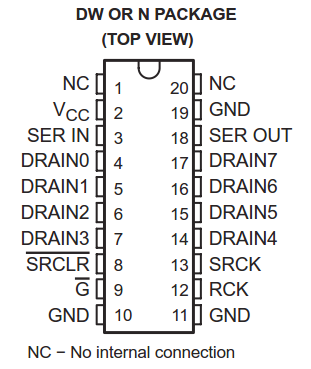
\includegraphics[width=0.3\textwidth]{figures/shift_reg.png}  & 
      {\begin{tabularx}{\cellwidth}{ lX  }      
      $V_{cc}$ & Positive supply voltage\\
      GND & Ground \\
      SER IN & Daten Pin \\
      SRCK & Clock Pin \\
      RCK & Latch Pin \\
      $\overline{SRCLR}$ & Wenn \textbf{shift-register clear} LOW ist, werden die input Register gelöscht\\
      $\overline{G}$ & Wenn \textbf{output enable} HIGH ist, werden die Daten im Output Buffer LOW gehalten
      \end{tabularx}   }
      \end{tabularx}
      \caption{Aufwändige Tabelle mit Abbildung und Caption}
      \label{tbl:shiftReg}
      \end{center}
\end{table}

Tabellen sind in Latex sehr kompliziert zu erzeugen. Alternativ kann man die Tabellen auch in einem anderen Programm gestalten und als Bild wieder einfügen. Dieses Bild kann dann innerhalb von begin-Table verwendet werden.

\section{Beispiele Listen}
Im Folgenden wird eine Liste gezeigt:
\begin{itemize}
  \item Ich weiß, dass viele Geräte des täglichen Lebens durch Computer
  gesteuert werden und kann für mich relevante nennen und nutzen.
  \begin{enumerate}
  	\item Und jetzt eine Numerierung
  	\item Und jetzt eine Numerierung
  \end{enumerate}
  \item Ich kann wichtige Bestandteile eines Computersystems (Eingabe-,
  Ausgabegeräte und Zentraleinheit) benennen, kann ihre Funktionen beschreiben
  und diese bedienen.
\end{itemize}

Und jetzt eine Numerierung:

\begin{enumerate}
	\item Aufzählungspunkt
	\begin{enumerate}
		\item Unteraufzählung
		\item Unteraufzählung
		\begin{itemize}
			\item Und jetzt noch eine Ebene ohne Aufzählung
			\item Und jetzt noch eine Ebene ohne Aufzählung
		\end{itemize}
	\end{enumerate}
	\item Aufzählungspunkt
	\item Aufzählungspunkt
	\item Aufzählungspunkt
	\item Aufzählungspunkt
\end{enumerate}

\section{Beispiel Codesequenz}
In \cref{code:qj} sieht man ein Quick-Sort-Listing in der Programmiersprache JAVA. Das Listings-Paket übernimmt die Formatierung von Codebausteinen und kann in der Präambel nach Belieben auf eine andere Sprache konfiguriert werden.

\def \currentAuthor {Author2}

\subsection{Quicksort in JAVA}
\begin{lstlisting}[language=Java, caption=QuickSort in Java, label=code:qj]
public class QuickSort {
public static void main(String[] args) {
int[] x = { 9, 2, 4, 7, 3, 7, 10 };
System.out.println(Arrays.toString(x));

int low = 0;
int high = x.length - 1;

quickSort(x, low, high);
System.out.println(Arrays.toString(x));
}

public static void quickSort(int[] arr, int low, int high) {
if (arr == null || arr.length == 0)
return;

if (low >= high)
return;

// pick the pivot
int middle = low + (high - low) / 2;
int pivot = arr[middle];

// make left < pivot and right > pivot
int i = low, j = high;
while (i <= j) {
while (arr[i] < pivot) {
i++;
}

while (arr[j] > pivot) {
j--;
}

if (i <= j) {
int temp = arr[i];
arr[i] = arr[j];
arr[j] = temp;
i++;
j--;
}
}

// recursively sort two sub parts
if (low < j)
quickSort(arr, low, j);

if (high > i)
quickSort(arr, i, high);
}
}
\end{lstlisting}

\section{Beispieltext}

\Blindtext

\listoffigures

\listoftables

\lstlistoflistings

\bibliographystyle{dinat}
%\bibliographystyle{plainurl}
\bibliography{Literatur_Verzeichnis} 

\appendix
\chapter{Anhang-Kapitel}
\section{Anhang-Section}
Testtext

\end{document}